\documentclass[10pt]{article}
\usepackage[polish]{babel}
\usepackage[utf8]{inputenc}
\usepackage[T1]{fontenc}
\usepackage{amsmath}
\usepackage{amsfonts}
\usepackage{amssymb}
\usepackage[version=4]{mhchem}
\usepackage{stmaryrd}
\usepackage{graphicx}
\usepackage[export]{adjustbox}
\graphicspath{ {./images/} }

\title{GIMNAZJUM }

\author{}
\date{}


\begin{document}
\maketitle
\begin{enumerate}
  \item Na okręgu umieszczono 2010 punktów białych i 1 punkt czerwony. Rozpatrujemy wszystkie możliwe wielokąty o wierzchołkach w tych punktach. Których wielokątów jest więcej: mających czerwony wierzchołek, czy mających tylko białe wierzchołki? Odpowiedź uzasadnij.
  \item Boki prostokąta mają długości 10 i 24. Przekątną podzielono ten prostokąt na dwa trójkąty. Oblicz odległość środków okręgów wpisanych w te trójkąty.
  \item Do dwóch okręgów stycznych zewnętrznie w punkcie \(A\) poprowadzono wspólną styczną \(B C\) (punkty \(B\) i \(C\) są punktami styczności). Udowodnij, że odcinki \(A B\) i \(A C\) są prostopadłe.\\
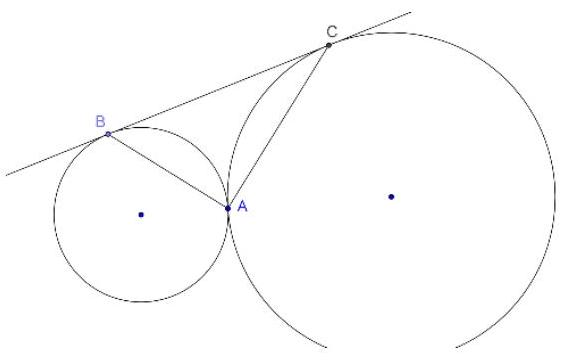
\includegraphics[max width=\textwidth, center]{2024_11_21_bbb3d86d6b5f62b4382ag-1}
\end{enumerate}

\section*{LICEUM}
\begin{enumerate}
  \item Przez wierzchołek \(A\) kwadratu \(A B C D\) poprowadzono prostą przecinającą przedłużenia boków \(B C\) i \(C D\) odpowiednio w punktach \(M\) i \(N\). Udowodnij, że:
\end{enumerate}

\[
\frac{1}{A M^{2}}+\frac{1}{A N^{2}}=\frac{1}{A B^{2}}
\]

\begin{enumerate}
  \setcounter{enumi}{1}
  \item Każde pole tablicy o wymiarach \(5 \times 5\) pomalowano albo na czarno, albo na biało. Wykaż, że można tak wybrać dwa wiersze i dwie kolumny tej tablicy, aby cztery pola na ich przecięciach były tego samego koloru.
  \item Znajdź wszystkie funkcje takie, ze dla dowolnych liczb rzeczywistych \(x, y\) spełniona jest równość
\end{enumerate}

\[
(f(x+y))^{2}=(f(x))^{2}+(f(y))^{2}
\]

Rozwiązania nalė̇y oddać do piątku 29 maja do godziny 12.30 koordynatorowi konkursu panu Jarostawowi Szczepaniakowi lub swojemu nauczycielowi matematyki.

Na stronie internetowej szkoły w zakładce Konkursy i olimpiady można znaleźć wyniki dotychczasowych rund i rozwiązania zadań.


\end{document}